\documentclass[12pt, oneside]{article} 
\usepackage{amsmath, amsthm, amssymb, calrsfs, wasysym, verbatim, bbm, color, graphics, geometry}
\usepackage{mathtools}
\usepackage{hyperref}

\geometry{tmargin=.75in, bmargin=.75in, lmargin=.75in, rmargin = .75in}  
\setlength{\parindent}{0in}
\setlength{\parskip}{\baselineskip}%
\setlength{\parindent}{1.5pt}%

\newcommand{\R}{\mathbb{R}}
\newcommand{\C}{\mathbb{C}}
\newcommand{\Z}{\mathbb{Z}}
\newcommand{\N}{\mathbb{N}}
\newcommand{\Q}{\mathbb{Q}}
\newcommand{\Cdot}{\boldsymbol{\cdot}}
\newcommand{\block}[1]{
  \underbrace{\begin{matrix}1 & \cdots & 1\end{matrix}}_{#1}
}
\newtheorem{thm}{Theorem}
\newtheorem{defn}{Definition}
\newtheorem{conv}{Convention}
\newtheorem{rem}{Remark}
\newtheorem{lem}{Lemma}
\newtheorem{cor}{Corollary}
\usepackage{tikz}  %TikZ central library is called.
\usetikzlibrary{automata,positioning} 
\usepackage{standalone}
\usepackage{pdfpages}

\tikzset{%
  every neuron/.style={
    circle,
    draw,
    minimum size=0.8cm
  },
  neuron missing/.style={
    draw=none, 
    scale=2,
    text height=0.2cm,
    execute at begin node=\color{black}$\vdots$
  },
  arro/.style={
    ->,
    >=latex
  },
  bloque/.style={
    draw,
    minimum height=1cm,
    minimum width=0.5cm
  }  
}


\title{Lecture Note - 07: Neural Network}
\author{Dihui Lai}

\begin{document}


\maketitle
\tableofcontents

\vspace{.25in}

\section{A Single Neuron}

An artificial neuron is the basic computing unit in an artificial neural network. There are different way to define a neuron. The most common one is shown in Figure 1.
\begin{figure}
\center
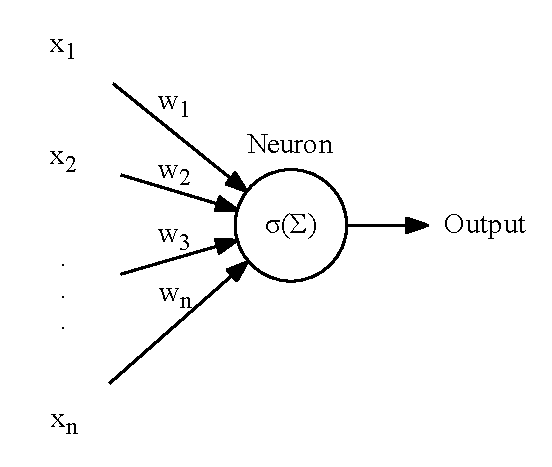
\includegraphics[scale=0.6,page=1]{Figures/singleneuron.pdf}
\caption{Schema: a single neuron with activation function $\sigma$}
\end{figure}

\subsection{Input}
A neuron receives multiple inputs $x_1$, $x_2$, ..., $x_n$. The signals are summed up after modulated by a set of weights $w_1$, $w_2$, ... $w_n$. Let us denote the weighted sum $z$
\begin{equation}
z=\sum\limits_{i=1}^{n}w_i x_i
\end{equation}

Usually a biased term $w_0$ is added to the summation and we have 
\begin{equation}
z=\sum\limits_{i=1}^{n}w_i x_i+w_0
\end{equation}

\subsection{Output}
The weighted sum is further transferred via an activation function $\sigma$ and becomes the final output of the neuron
\begin{equation}
a=\sigma(z)=\sigma(\sum\limits_{i=1}^{n}w_i x_i+w_0)
\end{equation}

\subsection{Activation Function}
The activation function can of different types.  Below is a list of common activation functions. Almost all activation functions have an S-shape except for the ReLu function.
\begin{center}
\bgroup
\def\arraystretch{2.5}% 
\begin{tabular}{c|c} 
Name & Definition\\
\hline
Step Function & $\sigma (z)={\begin{cases}0&{\text{for }}z<0\\1&{\text{for }}z\geq 0\end{cases}}$\\
\hline
Logistic or sigmoid & $\sigma(z)={\frac {1}{1+e^{-z}}}$\\
\hline
hyperbolic tangent &$\sigma(z)={\frac {(e^{z}-e^{-z})}{(e^{z}+e^{-z})}}$\\
\hline
ReLU & $\sigma(z)=\begin{cases}0&{\text{for }}z\leq 0\\z&{\text{for }}z>0\end{cases}$
\end{tabular}
\egroup
\end{center}


\section{Neural Network}
\subsection{Forward Path}
Each neuron at layer ${l}$ receives inputs from all neuron from the previous layer ${l-1}$,
\begin{equation}
{z_k^l=\sum_jw^{l-1}_{kj}a_j^{l-1}}
\end{equation}
Here, $a_j^{l-1}$ is the input from $jth$ neuron from $l-1$ layer. The neurons transfer the input signal $z_k^l$ via a transfer function $\sigma$ and send as input to to the next layer
\begin{equation}
a_k^l=\sigma(z_k^l)
\end{equation}

Inserting equation (4) to (5), we have 
\begin{equation}
z_k^l=\sum_jw^{l-1}_{kj}\sigma(z_j^{l-1})=\sum_jw^{l-1}_{kj}a_j^{l-1}
\end{equation}

\begin{figure}
\center
\includestandalone[width=.6\textwidth]{Figures/neuralnetwork}
\caption{A neural network of multiple layer structures. The hidden layers before layer $l-1$ and after layer $l$ are not shown. }
\end{figure}


\subsection{The Derivatives of Neural Network}
In order to calculate the neural network properly we need to understand a few derivatives.

\begin{itemize}
\item The partial derivatives of $z^{l}_k$ against $z^{l-1}_j$
\begin{equation}
\frac{\partial z^{l}_k}{\partial z_j^{l-1}}=w^{l-1}_{kj}\sigma'(z^{l-1}_j)
\end{equation}

\item The partial derivatives of $z^{l}_k$ against a weight element $w_{kj}^{l-1}$
\begin{equation}
\frac{\partial z^{l}_k}{\partial w_{kj}^{l-1}}=\sigma(z^{l-1}_j)
\end{equation}

\item Given a function of $f(z^{l-1}_j)$, we can explicitly express it in terms of $z^{l}$s,
$$
f(z^{l-1}_j)=f(z^l_1(z^{l-1}_j), z^l_2(z^{l-1}_j)...z^l_m(z^{l-1}_j)...)
$$
its derivative w.r.t $z^{l-1}_j$ is
\begin{equation}
\frac{\partial f}{\partial z^{l-1}_j}=\sum\limits_m \frac{\partial f}{\partial z^{l}_m}\frac{\partial z^l_m}{\partial z^{l-1}_j}=\sum\limits_m \frac{\partial f}{\partial z^{l}_m}w^{l-1}_{mj}\sigma'(z^{l-1}_j)
\end{equation}

\end{itemize}



\subsection{Backpropagation}
Consider neural network that has N layers, the cost function is dependent on all the $z$s of neurons in all layers
\begin{equation}
C\left(\vec{z}^N(\vec{z}^{N-1}(...\vec{z}^{l}(\vec{z}^{l-1})...) ...\vec{z}^1)\right)
\end{equation}

In order to find the weights that optimiaze the cost function, we can use gradient descent. Recall the gradient descent methods updates weights of layer $l-1$ as of the following

\begin{equation}
w_{kj}^{l-1} \leftarrow w_{kj}^{l-1}-\eta \frac{\partial C}{\partial w_{kj}^{l-1}}
\end{equation}

By using the chain rule, we have 
\begin{equation}
\frac{\partial C}{\partial w_{kj}^{l-1}}
=\frac{\partial C(...(z^l_k(w_{kj}^{l-1},...)))}{\partial w_{kj}^{l-1}}
=\frac{\partial C}{\partial z_k^l}\frac{\partial z_k^l}{\partial w_{kj}^{l-1}}
\end{equation}

There are two terms on the R.H.S. of the equation, 

\begin{itemize}

\item Using equation (9), the first term becomes 
\begin{align*}
\frac{\partial C}{\partial z_k^l}=\sum_m \frac{\partial C}{\partial z_m^{l+1}} w^l_{mk}\sigma'(z_k^l)
\end{align*}
Use notation $\delta^l_k=\frac{\partial C}{\partial z_k^l}$ for short, we have
\begin{equation}
\delta^l_k=\sum_m \delta^{l+1}_m w^l_{mk}\sigma'(z_k^l)
\end{equation}

\item Using what we calculated in equation (8), the second term is simply the output from $jth$ neuron in layer $l-1$ 
\begin{equation}
\frac{\partial z_k^l}{\partial w_{kj}^{l-1}}=\sigma({z^{l-1}_j})=a^{l-1}_j
\end{equation}

\end{itemize}


Finally, we get our iteration methods for calculating the gradient of the cost function w.r.t the weights i.e.

\begin{equation}
\frac{\partial C}{\partial w_{kj}^{l-1}}=\delta_k^{l}a_j^{l-1}
\end{equation}

\section{Neural Network Training Algorithm}
So the overall backpropagation algorithm works as the following:

\begin{itemize}
\item Initialize all weights $w_{mk}^l$ in every layer of the neural network
\item Feedfoward: use formula (6) to caculate the quantities $z_k^l$, $a_k^l$ for each neuron in all layers. Note in the input layer $a_k=x_k$, $x_k$ are he inputs to the $1st$ layer neurons
\item Backpropagation: after calculating the feedforward path, we use the backpropagation to figure out all the $\delta_k^l$ and update the weights. In contrast to the forward path. The back propagation starts by calculating the $\delta_k^L$ of the last layer $L$. The $\delta_k^l$ is then iteratively calculated using equation (13).
\item Calculate the gradient of the cost function w.r.t to all weights $w_{kj}^{l-1}$
\item updates the weights using equation (11)

\end{itemize}


\end{document}

